\documentclass[12pt,a4paper]{article}
\usepackage[left=2.5cm,right=2.5cm,top=2.5cm,bottom=2.5cm]{geometry}
\usepackage[utf8]{inputenc}
\usepackage{amssymb, amsmath, amsthm}
\usepackage{graphics, graphicx}
\usepackage{hyperref}
\graphicspath{{./6.9/}}
\pagestyle{empty}
\hypersetup{
  colorlinks   = true, %Colours links instead of ugly boxes
  urlcolor     = blue, %Colour for external hyperlinks
}
\begin{document}
\textbf{Chapter 6 solutions  \hfill Hanna Gábor}\\

\begin{enumerate}
\item
\textit{If V changes during the episode, then (6.6) only holds approximately; what
would the difference be between the two sides? Let $V_t$ denote the array of state values
used at time t in the TD error (6.5) and in the TD update (6.2). Redo the derivation
above to determine the additional amount that must be added to the sum of TD errors
in order to equal the Monte Carlo error.}

\begin{align*}
G_t - V_t(S_t) & = R_{t + 1} + \gamma G_{t + 1} - V_t(S_t) + \gamma V_t(S_{t + 1}) -
\gamma V_t(S_{t + 1}) + \gamma V_{t + 1}(S_{t + 1})\\
& - \gamma V_{t + 1}(S_{t + 1})\\
& = (R_{t + 1} + \gamma V_t(S_{t + 1}) - V_t(S_t)) + (\gamma G_{t + 1} - \gamma V_{t + 1}(S_{t + 1}))\\
& + (\gamma V_{t + 1}(S_{t + 1}) -\gamma V_t(S_{t + 1}))\\
& = \delta_t + \gamma(G_{t + 1} - V_{t + 1}(S_{t + 1})) + \gamma \alpha \delta_{t + 1}\\
& = \delta_t + \gamma \alpha \delta_{t + 1} + \gamma \delta_{t + 1} + \gamma^2 \alpha \delta_{t + 2} + \gamma^2(G_{t + 2} - V_{t + 2}(S_{t + 2})) = \dots\\
& = \sum\limits_{k = t}^{T - 1} \gamma^{k-t}( 1 + \alpha) \delta_{k}
\end{align*}

\item
\textit{This is an exercise to help develop your intuition about why TD methods
are often more efficient than Monte Carlo methods. Consider the driving home example
and how it is addressed by TD and Monte Carlo methods. Can you imagine a scenario
in which a TD update would be better on average than a Monte Carlo update? Give
an example scenario—a description of past experience and a current state—in which
you would expect the TD update to be better. Here’s a hint: Suppose you have lots
of experience driving home from work. Then you move to a new building and a new
parking lot (but you still enter the highway at the same place). Now you are starting
to learn predictions for the new building. Can you see why TD updates are likely to be
much better, at least initially, in this case? Might the same sort of thing happen in the
original scenario?}

I can't really see it.

I have lots of experience, so the estimates that are made after I reached
the highway are quite accurate, there will be only small updates for those.
For the estimate before I reach the highway, the two update rules just give
approximately the same. I can't see a big difference before that, either.

\item
\textit{From the results shown in the left graph of the random walk example it
appears that the first episode results in a change in only V(A). What does this tell you
about what happened on the first episode? Why was only the estimate for this one state
changed? By exactly how much was it changed?}

The first episode must have terminated on the left with a reward of $0$.

The other state values didn't change because the error in those cases was\\
$R_{t + 1} + \gamma V(S_{t + 1}) - V(S_t) = 0 + 1 \cdot 0.5 - 0.5 = 0$.

$v(A)$ changed by $\alpha (R_{t + 1} + \gamma V(S_{t + 1}) - V(S_t)) = 0.1 (0 + 0 - 0.5) = -0.05$.

\item
\textit{The specific results shown in the right graph of the random walk example
are dependent on the value of the step-size parameter, $\alpha$. Do you think the conclusions
about which algorithm is better would be affected if a wider range of $\alpha$ values were used?
Is there a different, fixed value of $\alpha$ at which either algorithm would have performed
significantly better than shown? Why or why not?}

I don't think a wider range of $\alpha$ values would have a significant effect on the results.

\begin{itemize}
\item \textbf{Monte Carlo methods.}
The Monte Carlo version with $\alpha = 0.4$ starts to oscillate pretty fast and doesn't
seem to decrease. I expect a Monte Carlo method with a bigger $\alpha$ value to oscillate
around an error level which is at least as high as the error in the $\alpha = 0.4$
case. The smallest $\alpha$ for the MC method among the examples is $0.1$. That is
the only MC method which we can't see oscillate. This version does not achieve the
performance of the TD methods. A smaller $\alpha$ value would make the learning progress
even slower. It's possible that the error using Monte Carlo update with $\alpha =<0.1$
goes under the TD error eventually, but it would still be pretty slow.

\item \textbf{TD methods.}
The TD version with $\alpha = 1.5$ plateaued fast at a relatively high error. I expect
bigger $\alpha$ values to make the convergence faster, but plateaue at a higher value.
The version with $\alpha = 0.5$ is the best among all shown algorithms. A TD method with a smaller
$\alpha$ value might reach an even lower error, but the $\alpha = 0.5$ case is already pretty good.
\end{itemize}

\item
\textit{In the right graph of the random walk example, the RMS error of the
TD method seems to go down and then up again, particularly at high $\alpha$’s. What could
have caused this? Do you think this always occurs, or might it be a function of how the
approximate value function was initialized?}

I think what causes this is the following. Suppose our current estimates are the real values and e.g.
we reach state $E$. Depending on our next step, $V_t(E)$ might take a small step in
the direction of $V_{t - 1}(D)$ or $1$. But you can only reach $E$ from $D$,
so $V_t(D)$ will be bigger than $V_{t - 1}(D)$. This means that the expected value
of $V_{t + 1}(E)$ will be closer to $1$ than to $V_{t - 1}(D)$. This means that the
equilibrium for $V_t(E)$ is a bit bigger than the real $V(E)$. The smaller
the $\alpha$ is, the closer the equilibrium is to the real value.

If we have started with a higher initial value for $D$ and $E$ than the true value
and a lower initial value for $A$ and $B$, then I wouldn't expect to see this increase
in the error.

\item
\textit{In Example 6.2 we stated that the true values for the random walk example are
$\frac{1}{6}, \frac{2}{6}, \frac{3}{6}, \frac{4}{6}, \frac{5}{6}$, for states A through E.
Describe at least two different ways that these could have been computed. Which would
you guess we actually used? Why?}

A fast method is the following. $v(S) = 0.5 \cdot v(S_l) + 0.5 \cdot v(S_r)$, where $S_l$ is the
left neighbor of $S$ and $S_r$ is the right neighbor of $S$. This means that $v(S) - v(S_l) = v(S_r) - v(S)$. Hence, the numbers $0 \le v(A) \le v(B) \le v(C) \le v(D) \le v(E) \le 1$ are equidistant, so
each difference is $\frac{1}{6}$.

A slightly different method is to write down these five equations and solve the resulting
linear equation system.

\item
\textit{Design an off-policy version of the TD(0) update that can be used with
arbitrary target policy $\pi$ and covering behavior policy b, using at each step t the importance
sampling ratio $\rho_{t:t}$ (5.3).}

I would use the update rule:
\[V(S_t) \leftarrow V(S_t) + \alpha \rho_{t:t} (R_{t + 1} + \gamma V(S_{t + 1}) - V(S_t)).\]

\item
\textit{Show that an action-value version of (6.6) holds for the action-value form
of the TD error $\delta_t = R_{t+1} + Q(S_{t+1}, A_{t+1}) - Q(S_t, A_t)$, again
assuming that the values don’t change from step to step.}

It's basically the same, we just change $V(S_t)$ to $Q(S_t, A_t)$:

\begin{align*}
  G_t - Q(S_t, A_t) &= R_{t + 1} + \gamma G_{t + 1} - Q(S_t, A_t)
  + \gamma Q(S_{t + 1}, A_{t + 1}) - \gamma Q(S_{t + 1}, A_{t + 1})\\
  &= \delta_t + \gamma (G_{t + 1} - Q(S_{t + 1}, A_{t + 1}) = \dots \\
  &= \sum\limits_{k = t}^{T - 1} \gamma^{k - t} \delta_k
\end{align*}

\item
\textit{Windy Gridworld with King’s Moves. (Programming.) Re-solve the windy
gridworld assuming eight possible actions, including the diagonal moves, rather than four.
How much better can you do with the extra actions? Can you do even better by including
a ninth action that causes no movement at all other than that caused by the wind?}

The ninth action doesn't help, the minimum number of steps is also available with
eight options. As there are more possibilities, it makes the learning a bit slower.

The code can be found \href{https://github.com/hannagabor/SBRL}{here}.

\begin{center}
  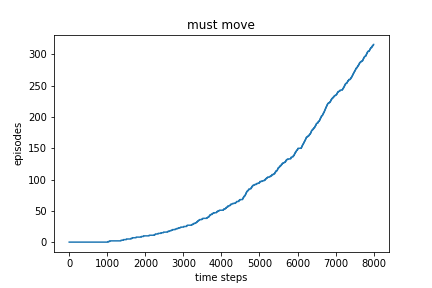
\includegraphics[scale=0.8]{must_move_plot}
  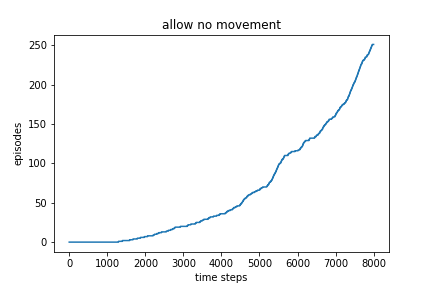
\includegraphics[scale=0.8]{no_movement_plot}
\end{center}

Example trajectory:

\begin{center}
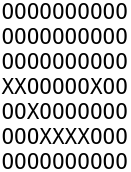
\includegraphics[scale=0.5]{trajectory}
\end{center}

\item
\textit{Stochastic Wind. (Programming.) Re-solve the windy gridworld task with
King’s moves, assuming that the effect of the wind, if there is any, is stochastic, sometimes
varying by 1 from the mean values given for each column. That is, a third of the time
you move exactly according to these values, as in the previous exercise, but also a third
of the time you move one cell above that, and another third of the time you move one
cell below that. For example, if you are one cell to the right of the goal and you move
left, then one-third of the time you move one cell above the goal, one-third of the time
you move two cells above the goal, and one-third of the time you move to the goal.}

Apparently, this makes the problem much more difficult. The code can be found \href{https://github.com/hannagabor/SBRL/blob/6.9/windy_gridworld.ipynb}{here}.

\begin{center}
  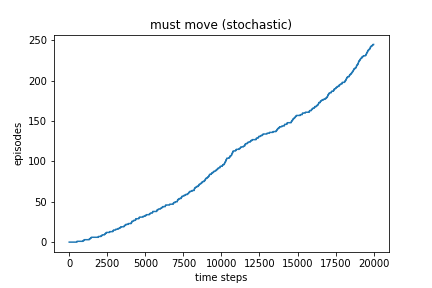
\includegraphics[scale=0.8]{stochastic_must_move_plot}
  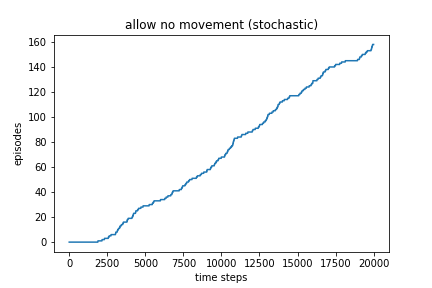
\includegraphics[scale=0.8]{stochastic_no_movement_plot}
\end{center}

An example trajectory:
\begin{center}
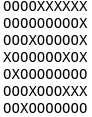
\includegraphics[scale=0.8]{stochastic_trajectory}
\end{center}

\end{enumerate}
\end{document}
